\documentclass[12pt,a4paper,ngerman]{scrartcl}
\usepackage[left=2.5cm,right=2.5cm,top=1cm,bottom=2cm,includeheadfoot]{geometry}
\usepackage{babel}
\usepackage[T1]{fontenc}
\usepackage{verbatim} %muss vorhanden sein für \begin{comment}
\usepackage{amsmath}
\usepackage{amssymb}
\usepackage[utf8]{inputenc}
\usepackage{graphicx}

\usepackage{enumitem}

\usepackage[super,square,comma]{natbib}

\usepackage{hyperref}
\hypersetup{
	%linktocpage,
	colorlinks,
	citecolor=black,
	filecolor=black,
	linkcolor=black,
	urlcolor=black}

\makeatletter
\renewcommand\paragraph{\@startsection{paragraph}{4}{\z@}%
  {-3.25ex\@plus -1ex \@minus -.2ex}%
  {1ex \@plus .2ex}%
  {\normalfont\normalsize\bfseries}}
\makeatother

\usepackage[usenames,dvipsnames]{color}
\usepackage{listings}
\lstset{
    backgroundcolor=\color[rgb]{0.95,0.95,0.95},
    columns=flexible, 
    numbers=left, 
    numbersep=5pt, 
    numberstyle=\scriptsize, 
    basicstyle=\ttfamily\footnotesize,
    captionpos=b,
    keywordstyle=\color{Mahogany},
    commentstyle=\color[rgb]{0.133,0.545,0.133},
    stringstyle=\color{MidnightBlue},
    breaklines=true,
    frame=shadowbox,
    rulesepcolor=\color[rgb]{0.7,0.7,0.7} % color of box-shadow
}

\usepackage{xcolor}

\usepackage{float}
\usepackage{parskip}
%\usepackage[none]{hyphenat}



\begin{document}

\begin{titlepage}

\vspace*{3 cm}

\begin{flushright}

\bfseries{\Huge\scshape Jonglieren mit der Kinect\\{\Large ein Softwareprojekt im}\\Projekt Bildverarbeitung}
\end{flushright}

\vspace{2 cm}

\begin{flushright}
\scshape{\large Projektbericht}
\end{flushright}

\begin{flushright}
\scshape{\LARGE\bfseries Rolf Boomgaarden\\}
\scshape{\LARGE\bfseries Florian Letsch\\}
\scshape{\LARGE\bfseries Thiemo Gries\\}
\end{flushright}

\vspace{2 cm}

\begin{flushright}
\scshape{\large\bfseries \today}
\end{flushright}

\vfill

\begin{flushright}

\scshape{Unter Aufsicht von: {\bfseries Benjamin Seppke}\\}
\scshape{\bfseries Arbeitsbereich Kognitive Systeme\\}
\scshape{\bfseries Fachbereich Informatik, Universität Hamburg\\}
\end{flushright}

\end{titlepage}

\tableofcontents
\newpage

\section{Einleitung}

Lorem ipsum dolor sit amet, consectetur adipiscing elit. Sed aliquam, ligula vitae condimentum malesuada, turpis nisi placerat eros, vel facilisis mi neque quis nulla. Aenean eleifend risus id dolor ultricies scelerisque. Phasellus venenatis libero enim, vel lacinia massa interdum nec. Quisque a euismod ligula. In eget mattis orci. Integer vitae enim ac nisl scelerisque luctus ut et nibh. Quisque ut odio ultrices, consequat mi vel, accumsan metus. Donec faucibus, nulla vel mattis euismod, felis leo accumsan tortor, et congue turpis leo et elit. Proin gravida mollis facilisis. In enim nisi, pellentesque id tincidunt a, accumsan eget elit. Aliquam erat volutpat. In quam ante, accumsan eu est a, molestie euismod neque. Proin porta rhoncus nisl sed dignissim. Aliquam lacinia sed libero et eleifend. Ut placerat tortor eget augue pellentesque rutrum.

\section{Motivation}

Mit den technischen Möglichkeiten eines Tiefen- und Bilddaten liefernden Systems 
(konkret: Microsoft Kinect) soll in dieser Arbeit versucht werden, das Wurfmuster
eines mit Bällen jonglierenden Akteurs zu analysieren.

Ein Jongleur wirft Jonglierbälle in einem Muster, das möglichst gleichmäßig ist.
So ist der Höhepunkt der Flugbahn idealerweise konstant auf der gleichen Höhe.
Zum Analysieren des Jongliermusters wäre dies also bereits ein erstes Kriterium, 
die \textit{Güte eines Jongliermusters} automatisiert zu bewerten.

Denkbar sind auch weitere Anwendungen, wie etwa das automatische Zählen von 
erfolgreich gefangenen Würfen. Eine computergesteuerte Erfassung der insgesamten
Wurfzahl ist ein einfaches Kriterium für eine \textit{Leistungsbewertung des 
jonglierenden Benutzers}.

Die genaue Anwendung ist jedoch nicht Ziel dieser Arbeit. Stattdessen verfahren wir
in einem bottom-up Herangehen, um von den rohen Bild- und Tiefendaten der Kinect 
ausgehend Informationen über sich im Bild befindliche Objekte (Jonglierbälle) zu
erfassen und deren Bewegung zu erkennen. Das Ergebnis ist dann ein Fundament, auf
dessen Grundlage konkrete Anwendungen entwickelt werden können.

\section{Zielsetzung}

Am Ende dieser Arbeit soll eine Anwendung stehen, die mit Hilfe der Kinect Daten 
über die Flugbahnen dreier jonglierter Bälle liefert. 

Ein Akteur befindet sich hierbei im Bildzentrum in einem wohl definierten Abstand 
zur Kinect. Es werden drei matte Bälle beliebiger Farbe jongliert. Um das Ergebnis
unabhängig von der Szenenbeleuchtung zu halten, sollen die Tiefendaten ausreichend
Information für das eindeutige Identifizieren der Bälle liefern.

\section{Möglichkeiten der Kinect}

Die Kinect ist eine von Microsoft zur Spielekonsole Xbox 360 vertriebene Erweiterung,
die den Spieler mit einem RGB- und einem Tiefensensor erfasst und diese beiden 
Datenströme an die Konsole liefert. Da die Kinect über einen USB-Anschluss verfügt,
kann sie an konventionellen Rechnern angeschlossen und betrieben werden. Eine 
quelloffene Implementierung zur Unterstützung der Kinect ist das freenect Projekt,
das für Linux, Windows und MacOS zur Verfügung steht und im Rahmen dieser Arbeit
als Bibliothek für Python verwendet wurde.\cite{openkinect}\cite{libfreenect}

FIXME: Abbildung Kinect mit gelabelten Komponenten?

Die Videoquelle der Kinect liefert standardmäßig 30 Bilder pro Sekunde mit einer
Auflösung von 640x480 und 8 bit Farbtiefe. Tatsächlich kann sie mit
einer Auflösung von 640x512 aufnehmen (oder sogar 1280x1024 und 10 fps), aber die 
Auflösung wird an die der Tiefenkamera angepasst, so dass die reduzierte Auflösung 
ausgegeben wird. Die Tiefendaten stammen von einer 
Infrarot-Kamera und liefern bei gleicher Bildfrequenz 2048 verschiedene 
Tiefenwerte (11bit). Das Tiefenbild deckt einen Bereich von 0,8 m bis 3,5 m von der
Kinect aus ab, bei der in 2m Entfernung eine Auflösung von 3 mm in der Bildebene und
1 cm in der Tiefenebene erreicht wird. Aus der Funktionsweise der Infrarotkamera
ergibt sich, dass die Kinect in Umgebungen starker Infrarotstrahlung (beispielsweise
im Tageslicht) nur beschränkt einsatzfähig ist.\cite{hacking}

FIXME: Erklären wie das mit diesem projizierten Punktemuster funktioniert.

Um das Tiefenbild zu erhalten, besitzt die Kinect zwei Hardware-Komponenten, einen
Infrarot-Laser und eine Infrarot-Kamera. Der IR-Laser strahlt Licht mit einer Wellenlänge
von 830 nm, welches ein bekanntes Rausch-Muster erzeugt. Dieses Rausch-Muster enthält
mitunter neun hellere Punkte, die über das Muster verteilt sind.\\
Die Kinect nutzt die Streifenprojektion (auch Streifenlichttopometrie genannt), um ein
räumliches Bild zu erfassen. So wird das vom Laser erzeugte bekannte Rauschmuster mit der
in einem festen Abstand zum Laser befestigten IR-Kamera erfasst. Weicht das aufgenommene
Bild von dem bekannten Rausch-Muster ab, kann davon ausgegangen werden, dass dies durch
Objekte im Raum, die das Muster stören, verursacht wird. Mit Hilfe der helleren Punkten werden
alle Punkte zugeordnet und es kann ein räumliches Bild errechnet werden.

FIXME: Abbildung Rausch-Muster des IR-Lasers

Mögliche Störungen entstehen durch die Stärke der Laserdiode und der Wellenlänge des Lichts.
Die IR-Kamera der Kinect hat einen Infrarot-Pass-Filter, der nur Licht im Bereich von 830 nm
hindurch lässt, um nicht durch anderes Licht (wie beispielsweise Fernbedienungen) geblendet zu
werden. Dennoch gibt es Lichtquellen, wie das Sonnenlicht, welches genügend Licht mit einer
Wellenlänge von 830 nm  beinhaltet, um die Kinect blenden zu können. So kann bei starkem
Tageslicht oder im freien von Fehlverhalten bis zur Unnutzbarkeit der Kinect gerechet werden.

FIXME: Beispielkinectprojekte!

\section{Recherche: Ein jonglierender Roboter} 

Im Vorfeld der ersten eigenen Implementierungsversuche sind wir bei der 
Paper-Recherche auf eine Arbeit von FIXME gestoßen, die zumindest in Teilen
eine ähnliche Aufgabenstellung verfolgte. Unter dem Titel "Playing catch and juggling 
with a humanoid robot" untersuchte die Gruppe des Disney Research Center (FIXME)
einen humaoiden Roboter, der auf ihn zugeworfene Bälle fangen und zurückwerfen soll.
In der Entwicklung dieses Systems war ein Teil der Gesamtaufgabe ein 
bild- und tiefendatenverarbeitendes System, das mit einer der Kinect sehr ähnlichen
Kamera arbeitete.

Kernidee dieses Systems war eine \textit{Image Processing Pipeline}, also eine
Kette von Verarbeitungsschritten, die als Eingabe eine Folge von RGB- und Tiefendaten
nahm und als Ausgabe die aktuelle Position und zukünftige berechnete Flugbahn 
liefern. 

FIXME: Processing Pipeline

Die gelöste Aufgabe in dieser Arbeit ist also von der Grundidee her also eine ganz
ähnliche, weshalb wir den Grundaufbau der Verarbeitungsschritte auch in unserem 
Vorgehen übernehmen wollten. Wie wir im Laufe der Programmierung aber feststellten,
hatte die Arbeit einige Rahmenbedingungen anders gesetzt, so dass wir auf Probleme 
stießen, die sich in der Arbeit mit dem Roboter offensichtlich nicht so deutlich
gezeigt haben.

Hierbei ist zuerst zu nennen, dass die betrachteten Bälle bei uns sehr viel kleiner
waren, da wir einen tatsächlich jonglierenden Menschen betrachtet haben. In der
Arbeit mit dem Roboter wurden sehr große Bälle verwendet, die von den werfenden
Menschen mit beiden Händen gehalten und geworfen wurden.

Hierdurch ergeben sich auch längere Wurfbahnen, die tendenziell auch weiter 
auseinander liegen. Wie später in der Arbeit zu sehen sein wird, ist das normale
Jongliermuster mit zwei Händen teilweise so klein, dass es schwer wird, dicht 
aneinander vorbei fliegende Bälle voneinander zu unterscheiden.

Zusätzlich wurde in der Arbeit mit dem Roboter auf verschiedenfarbige Bälle 
zugegriffen, um diese voneinander zu unterscheiden. Dies ist eine Rahmenbedingung,
die wir so nicht wählen wollten, da die RGB-Werte, die die Kinect liefert, sehr stark 
von den Beleuchtungsbedingungen abhängen und bei den verschwischten Objekten, wie
wir sie in den Kinect-Aufnahmen sehen, keine robuste Erkennung zu ermöglichen 
versprechen.


\section{Lösungsidee}

Als erste Lösungsidee haben wir in Anlehnung an die betrachtete Arbeit mit dem 
jonglierenden Roboter eine eigene Zusammenstellung von durchzuführenden Bildverarbeitungsschritten erarbeitet wie in Abbildung FIXME zu sehen.

Die Verarbeitung wird auf den Einzelbildern durchgeführt, die Ergebnisse der 
einzelnen Bilder werden dann kombiniert.  

\begin{enumerate}
\item Auf den Tiefendaten werden ab einem bestimmten Tiefenwert (\textit{threshold}) 
	alle Tiefeninformationen abgeschnitten. Jongleur und fliegende Jonglierbälle sind
	somit freigestellt.
\item Auf den reduzierten Tiefendaten werden nun lokale Maxima bestimmt, welche die 
	Jonglierbälle sein müssen, da sie sich näher an der Kinect befinden als der 
	Jongleur. Hier sind auch die Hände enthalten.
\item Die gefundenen Maxima sind mögliche Kandidaten für tatsächlich erkannte 
	Jonglierbälle. 
\item Die entsprechenden Regionen werden als Maske für die RGB Daten verwendet.
\item In den interessanten Regionen der RGB Daten wird eine Erkennung für runde 
	Objekte durchgeführt. Dies wird mit einer \textit{Hough Transformation} gelöst.
\item Die nun erkannten Bälle werden aufgeteilt und den einzelnen Bällen zugeordnet.
\item Für jeden Ball liegt nun also eine Reihe von Positionen vor. Um zu einer 
	flüssigen Flugbewegung zu gelangen wird die Flugbahn jedes Balls mit Hilfe eines
	\textit{Kalman-Filters} modelliert und laufend aktualisiert. Mit dieser stetigen
	Positionsinformation kann die Position eines Balles also programmseitig jederzeit 
	abgefragt werden.
\end{enumerate}


% FIXME: label etc
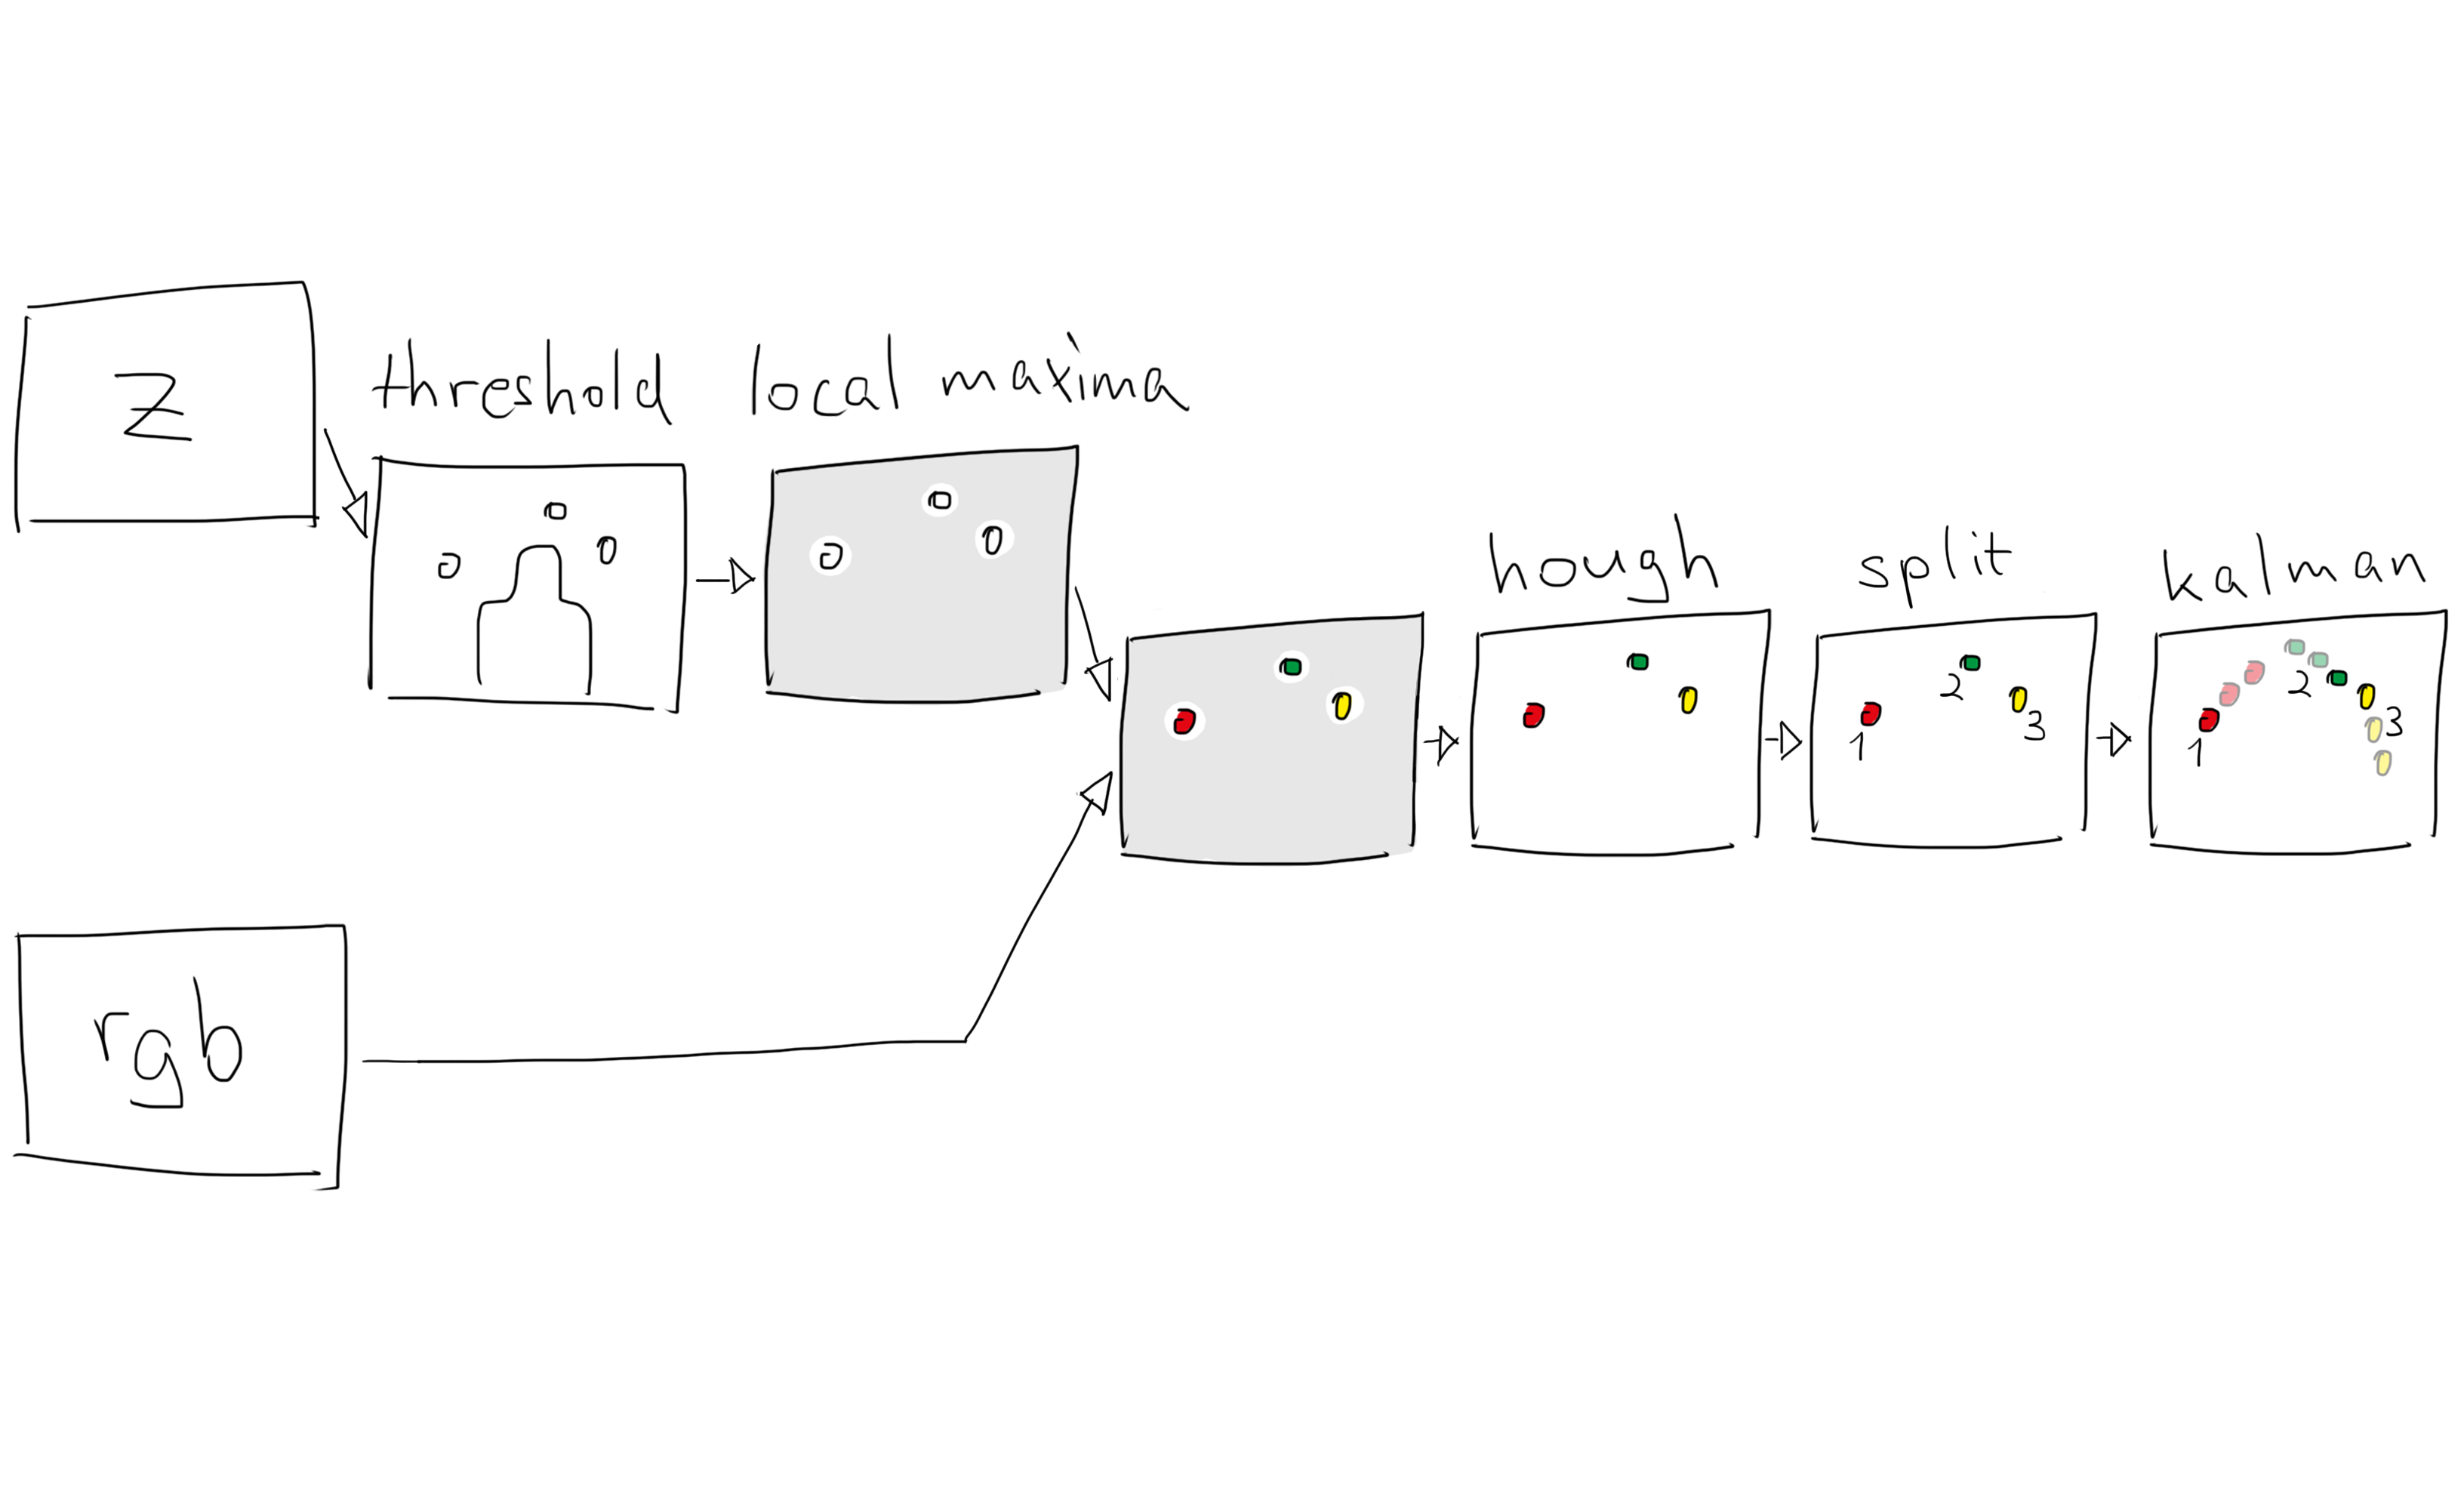
\includegraphics[scale=0.14]{img/processing-pipeline.png}

Wie sich im Laufe des Projektes heraus gestellt hat, ist diese Vorstellung der Arbeit 
auf den Echtzeitdaten in einigen Schritten zu idealisiert und in anderen unnötig 
kompliziert. Hierauf werden wir im finalen Schritt der Umsetzung eingehen.

\section{Umsetzung}

\subsection{Programmstruktur}

Die ersten Tests, die wir mit der Kinect und bildverarbeitenden Verfahren 
ausprobiert haben, bestanden aus wenigen Schritten und wurden in einer
simplen Schleife gelöst, die bei Druck der ESC Taste verlassen wurde. Zu Beginn
eines Schleifendurchlaufes wird ein neuer RGB Frame und die zugehörigen 
Tiefendaten geholt. Danach folgt schrittweise Verarbeitung dieser Daten je nach 
gewünschtem Zweck. 

FIXME: Einfacher Programmablauf, Blockdiagramm? Nur wenn wir noch Platz brauchen

Nun möchten wir je nach betrachtetem Arbeitsschritt aber verschiedene 
Verarbeitungsstufen ausführen oder ausklammern, so dass wir irgendwie eine
Parametrisierung finden mussten. Wir haben uns für ein Konzept von Filtern 
entschieden, wobei zu Programmstart eine Liste mit gewünschten Filtern erstellt
wird und diese in der Hauptschleife nacheinander ausgeführt werden (die Originaldaten
werden also in den ersten Filter gegeben, das Ergebnis dieses Filters wird als 
Eingabe für den zweiten Filter verwendet und das Ergebnis des letzten Filters
in der Liste wird dann als Gesamtausgabe visuell dargestellt.

Die RGB- und Tiefendaten werden vom freenect Modul als numpy Arrays zurückgegeben.
Die Ausgabe erfolgt über ein von OpenCV erzeugtes Fenster, welches Daten für 
OpenCV erwartet. Die numpy Arrays müssen also an einer Stelle umgewandelt werden.
Zusätzlich haben wir schnell festgestellt, dass einige gewünschte Operationen 
entweder nur in numpy oder nur in OpenCV zur Verfügung stehen. Ein mehrfaches 
Umwandeln von einem Format in das jeweils andere ist aus Performanz-Gründen 
natürlich zu vermeiden. Um in der Entwicklung nicht immer darauf achten zu müssen,
welcher Filter welche Eingabe erwartet und welche Ausgabe liefert, haben wir uns dazu
entschieden, jeden Filter als Eingabe Daten in numpy Darstellung zu liefern und auch
für die Ausgabe numpy zu erwarten. Dies erlaubt uns eine von außen identische 
Betrachtung der Filter, auch wenn einige Filter intern eine Umwandlung durchführen 
müssen. Bei etwaigen Problemen wollten wir die Performanz unserer Lösung getrennt
betrachten, um zu Beginn lediglich über eine funktionierende Lösung nachdenken
zu müssen.

Waren die Filter ursprünglich als isolierte Einheiten mit simplem 
Input-Output-Verhalten von Bild- bzw. Tiefendaten gedacht, fiel uns schnell auf,
dass einige Filter Zusatzinformationen liefern, die von anderen Filtern gebraucht 
werden. Um Filter nicht intern Unteraufrufe von von anderen Filtern oder Komponenten
ausführen zu lassen (dies wäre ebenfalls eine denkbare Lösung), entschieden wir uns
für ein Objekt, das von der Hauptkomponente des Programms in jeden Filter 
hineingereicht wird und in dem jeder Filter Informationen ablegen und abfragen kann.
Natürlich ist dies abhängig von der Reihenfolge der Filter und einige Filter haben 
als implizite Vorbedingung, dass andere Filter bereits ausgeführt wurden, dies haben
wir der Einfachheit halber aber nicht expliziert formuliert, im Zweifelsfall wird 
beim ersten Ausführen einer nicht korrekten Filterkombination oder -reihenfolge ein
Laufzeitfehler geworfen, da Informationen in dem übergebenen Objekt noch nicht 
vorhanden sind. Dieses Objekt ist ein schlichtes Python dictionary.


FIXME: Diagramm Programmstruktur (so cool skizziert, nicht ganz formell UML)

FIXME: bisschen Python Listing um diese Filter-Konzepte und das args dictionary zu zeigen


\subsection{Programmfluss}

\subsubsection{Schritt 1: Tiefendaten vorverarbeiten}

Normieren aux XXX Tiefenwerte

\subsubsection{Schritt 2: Regions Of Interest isolieren}

Hintergrund entfernen, Bälle freistellen. Zwei Ansätze:

A. keine Objekte auf Tiefenebene zwischen Spieler und Kinect, auch nicht am Rand. Tiefenwerte aber einem gewissen Wert einfach abschneiden. Annahme: Spieler steht auf Linie oder ähnlich. Tiefendaten binarisieren.

B. Mit temporalem Filtering sich bewegende Regionen isolieren. Erlaubt auch störende Objekte wie Stühle am Rand, Erfahrung aber nicht so gut, da das Verfahren bei schneller Bewegung (Ballwurf) nicht zuverlässig ist. Außerdem Probleme mit unscharfen Objekträndern und Rauschen. Außerdem technische Hürden (Vigra als weitere Abhängigkeit).

Bewertung: Ansatz A völlig ausreichend für unsere Zwecke. Einschränkung der Spielerposition nicht störend, da dies sogar interaktiv durchgeführt werden (so lange nach vorne gehen, bis System vernünftige Werte liefert - kein aufwändiges Abmessen nötig).

\subsubsection{Schritt 3: Bälle in Frame-Folgen einander zuordnen}

Bevor potentielle Ballpositionen konkreten Ball-Instanzen zugeordnet werden, findet eine kurze Vorverarbeitung statt, bei der Regionen im binarisierten Ergebnis des vorherigen Schrittes als Rechtecke umzeichnet werden, wofür einfach die OpenCV-Funktion \lstinline{cv.BoundingRect} verwendet wird, die genau diese Aufgabe erfüllt.
Kleine Rechtecke und solche, die den Bildrahmen berühren, werden hierbei bereits herausgefiltert.

Durch die resultierende Liste von Rechtecken wird iteriert und jeder 
Rechteckmittelpunkt als mögliche Ballposition aufgefasst (die kürzere Rechteckskante
wird vorerst als Balldurchmesser gespeichert, vorerst aber ignoriert). 

\begin{lstlisting}[language=Python,caption={RectsFilter.py, Ausschnitt}]
# ...

        storage = cv.CreateMemStorage(0)
        contour = cv.FindContours(depth_cv, storage, cv.CV_RETR_CCOMP, cv.CV_CHAIN_APPROX_SIMPLE)
        points = []

        ball_list = [] # collect ballpositions in loop
        while contour:
            x,y,w,h = cv.BoundingRect(list(contour))
            contour = contour.h_next()

            # filter out small and border touching rectangles
            t = 2 # tolerance threshold
            minsize = 5
            if x > t and y > t and x+w < self.WIDTH - t and y+h < self.HEIGHT - t and w > minsize and h > minsize:
                x -= 5
                y -= 5
                w += 10
                h += 10
                x, y = self._nullify(x), self._nullify(y) # why is this necessary now?

                ball_center = (x+w/2, y+h/2)
                ball_radius = min(w/2, h/2)
                ball_list.append(dict(position=ball_center, radius=ball_radius))

                # Draw rectancle with info
                cv.PutText(rgb_cv, '%d/%d' % (x, y), (x,y-2) , self.font, (0, 255, 0))
                cv.Rectangle(rgb_cv, (x, y), (x+w, y+h), cv.CV_RGB(0, 255,0), 2)

        args['balls'].addPositions(ball_list)
\end{lstlisting}

Es liegt nun
für jeden Frame eine Liste von möglichen Ballpositionen vor. Diese setzen sich 
zusammen aus tatsächlichen Ballpositionen, Positionen in denen sich die Hände befassen sowie potentiell weiteren Hindernissen im Sichtfeld der Kinect, wobei wir diese in unseren Testdaten vermeiden haben. Bei den tatsächlichen Ballpositionen ist zu beachten, dass diese etwas ungenau sind und mit mehreren Pixeln vom tatsächlichen Ballmittelpunkt abweichen können.

% FIXME: label etc
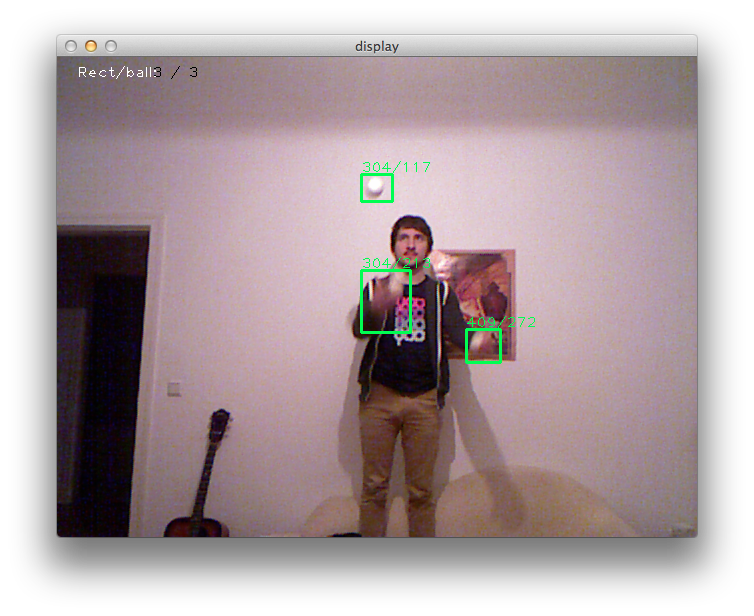
\includegraphics[scale=0.5]{img/rects-1.png}

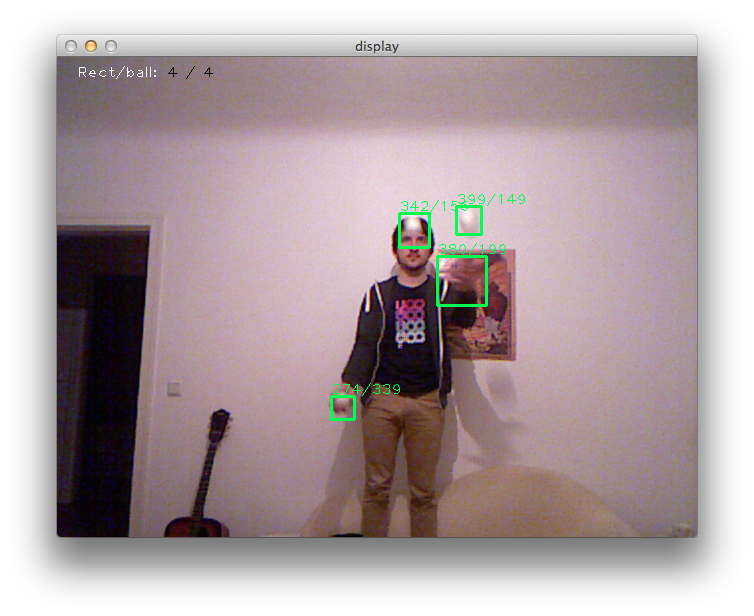
\includegraphics[scale=0.5]{img/rects-2.png}

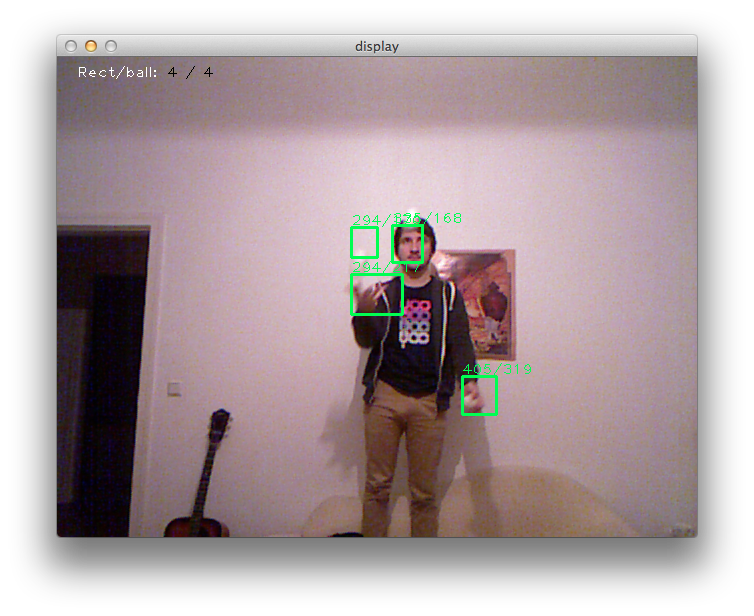
\includegraphics[scale=0.5]{img/rects-3.png}

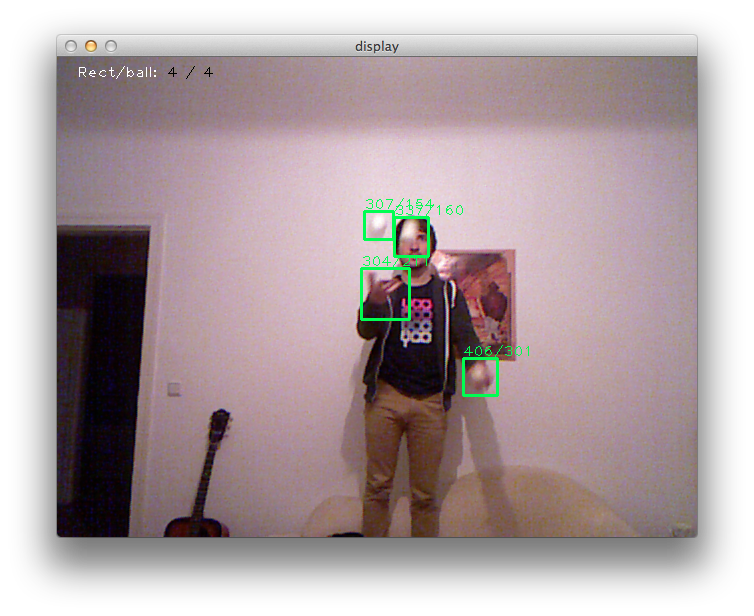
\includegraphics[scale=0.5]{img/rects-4.png}

Im Folgenden kommt die Hauptaufgabe dieses Schritts: Das Zuordnen der potentiellen
Punkte zu tatsächlichen Ballinstanzen, wobei diese Zuordnung über mehrere Frames 
hinweg eine neue Position einem bestehenden Ball zuordnen soll.

Dies ist der aufwändigste Schritt wie sich herausgestellt hat, zumindest der, mit dessen Lösung wir die meiste Zeit verbracht haben.

Als erste Idee, um falsche Positionen auszuschließen, dachten wir an eine 
Ballerkennung auf den RGB-Daten im Umfeld der Position. Naheliegend war die die 
Implementierung einer Hough-Transformation, mit der wir auch begonnen haben.
Erste Testläufe auf den RGB-Daten der Kinect zeigten aber, dass je nach Wahl der 
Parameter entweder die Bälle nicht erkannt, oder aber viel zu viele false-positives
erkannt wurden. Dies lag vor allem an den sehr verwischten Aufnahmen der Bälle 
während des Fluges. Bei Betrachtung der Beispielaufnahmen (siehe oben) wird auch 
deutlich, dass eine vermutete Position teilweise ein deutlich von der tatsächlichen
Position in den Bilddaten abwich. Somit konnten wir durch diesen Ansatz keinen Gewinn 
ziehen, so dass wir uns auch durch die Abweichungen zwischen Ballposition in RGB- udn 
Tiefendaten dazu entschlossen, uns alleine auf eine Untersuchung der Tiefendaten zu 
stützen.

Aber auch für die reine Berücksichtigung der Tiefendaten haben wir während des 
Projektablaufes mehrere Problemquellen identifizieren können, die die verschiedenen 
Ansätze unterschiedlich stark beeinflussen:

\begin{itemize}
 \item Hände sind auch als Rechtecke enthalten 
 \item Bälle fliegen sehr nah, teilweise überschneiden sich die Rechtecke zweier Bälle, so dass nur ein großes zu sehen ist und als eine mögliche Ballposition untersucht wird
 \item Ball legt in einem Frame (1/30 Sekunde) unterschiedlich lange Strecken zurück, teilweise sehr große (Pixelanzahl angeben?) 
 \item Mindestabstand zur Kinect resultiert in kleinem Jongliermuster, das verstärkt die problematischen Faktoren
 \item Teilweise fehlt eine Region in einem erkannten Frame
\end{itemize}
 
Diese Problemquellen wirken sich unterschiedlich stark auf die Eignung der von
uns im folgenden betrachteten Ansätze aus. Prinzipiell lassen sich die Ansätze
in zwei Gruppen unterteilen, in die erste Gruppe, bei der von vorneherein von einer
festen Ballanzahl ausgegangen wird und die zweiter Gruppe, der bei dynamisch auch wechselnde Ballanzahlen erlaubt sind.


Bei den Ansätzen mit fester Ballanzahl wird in jedem Verarbeitungsschritt versucht,
zu jeder bereits existierenden Ballinstanz eine Position aus den erkannten Rechtecken
auszuwählen, welche als neue Position des Balls erkannt wird. Da im Allgemeinen nie
zwei Bälle an der gleichen Position sein können, wird dieses Rechteck dann für die weiteren Ballinstanzen nicht mehr betrachtet, wir nennen die folgenden Ansätze daher
auch \textit{konsumierende Ansätze}. FIXME: das ist falsch, konsumierend $\neq$ feste Ballanzahl.
 
 \begin{enumerate}
 \item Nächste Punkte in zwei aufeinander folgenden Frames werden als der identische Ball aufgefasst. Nicht so zuverlässig, vor allem wegen schneller Ballbewegung und nah aneinander fliegender Bälle. Schwierig auch, wenn ein erkannter Ball fehlt -> Beachtung von "springenden" Bällen.
 \item Verbesserungsansatz: erwartete Ballposition wird approximiert mit vorheriger Bewegung (linearer Bewegungsvektor). Teilweise besser, aber schwierig, die initiale Bewegung zu Erkennen, auch weiterhin Probleme mit Lücken in den Informationen.
 \item Verbesserung: Nicht linear, sondern Flugbahn vorberechnen. Linearer Bewegungsvektor wird als Tangente an Steigung der Wurfparabel zu Grunde gelegt. (Verbesserung nochtmal gut angucken, aber gefühlt hat das erstaunlich wenig unterschied gebracht)
  \end{enumerate}
  
  
Im Gegensatz dazu sind die folgenden nicht konsumierende Ansätze zu sehen, bei denen
wir auch eine variable Ballanzahl erlauben. FIXME: das ist falsch, siehe oben
  
\begin{enumerate}
	\item wenn langsame Aufwärtsbewegung in aufeinander folgenden Frames erkannt wird: als Beginn eines Wurfes auffassen und an dieser Stelle einen Ball mit identischer Geschwindigkeit starten und dessen Flugbahn ab dort schrittweise simulieren. In jedem Schritt mit aktuell vorhandenen Bällen abgleichen und Wurfparameter anpassen. (hier schrittweise Bilder zeigen: Feuerwerk etc)
	\item wie Ansatz davor, allerdings wird die Parabel nicht approximiert, sondern
	aus den letzten 3 Frames berechnet mit \lstinline{np.polyfit}.
\end{enumerate}


\subsubsection{Schritt 4: Bereinigte Wurfparabel}

Das fehlt uns noch. Aber aus den gelieferten Daten wollen wir dann höher-levelige Informationen abstrahieren. Objektanzahl, Wurfhöhen, Würfe zählen, etc.

\subsection{Erläuterung verwendeter Bildverarbeitungsverfahren}

\subsubsection{Kalman Filter}

{\color{red} FIXME: alles überarbeiten, mehr, nochmal nachlesen, wie's wirklich ist, Schaubilder}

Der Kalman Filter kann sich bewegende Objekte beobachten und Schätzungen zur aktuellen oder auch zukünftigen Position machen.

In diesem Projekt wird er dazu verwendet, die Bälle zu beobachten und die weitere Flugbahn zu bestimmen. Damit kann eine voraussichtliche Flugbahn in die Ausgabe gezeichnet werden, aber auch in der internen Verfolgung und Zuordnung der Bälle spielen die Ergebnisse eine wichtige Rolle.

Der Kalman Filter besteht aus zwei Funktionen, einem {\tt predict} und einem {\tt update}. Im {\tt predict} wird mit Informationen zur Art der Bewegung und mit mindestens einer Ortsinformation zum Zeitpunkt {\tt t} eine Schätzung zum Ort im Zeitpunkt {\tt t+1} gemacht. Ein {\tt predict} kann beliebig oft hintereinander ausgeführt werden.

Im {\tt update} wird die aktuell gespeicherte Ortsinformation mit extern gewonnen Daten aktualisiert. Die hier gemessene Abweichung zwischen Schätzung und tatsächlichen Daten kann natürlich auch zur weiteren Schätzung eingebracht werden. Ein {\tt update} wird nicht mehrmals hintereinander ausgeführt.

\subsection{Herausforderungen}

Probleme aus den Ansätzen noch mal aufgreifen. Noch irgendwas abstrakteres dazu schreiben? Vielleicht dass wir uns nicht doll genug getracked haben dier Projektzeit über?

\subsection{Bewertung der Umsetzung}

Robustheit.

  - Position des Jongleurs (Bildzentrum VS Bildrand. Abstand zur Kinect)
  
  - Objekte am Bildrand (bewegte vs nicht bewegte)
  
  - Ungleichmäßiges Jongliermuster
  
  - Variation der Bälleanzahl

Effizienz. Speedup-Möglichkeiten?

Anwendungsrelevanz.

\section{Anwendungsmöglichkeiten}

Projekte nehmen als Grundlage für einfache Programme / Spiele.

\subsection{Objekte zählen}

Mit den erkannten momentan fliegenden Objekten haben wir als erste Anwendung einen
einfachen Zähler geschrieben, der die tatsächliche Anzahl der im Muster befindlichen Objekte zu bestimmen versucht.

Denke wäre eine Verfolgung der Objekte über einen längeren Zeitraum, um auch 
unabhängig voneinander erkannte Objekte in ihrer Identität zu bestimmen. Tatsächlich
ist ein deutlich simplerer Ansatz aber bereits sehr effektiv, indem über eine 
längere Anzahl Frames geschaut wird, wie viele Objekte in der Luft sind. Es wird der 
Durchschnitt dieser Werte gebildet und aufgerundet. Auf diesen Wert wird dann noch 
$1$ addiert, um zur tatsächlichen Anzahl zu gelangen. Dies ist der Tatsache 
geschuldet, dass beim normalen Jongliermuster zu jeder Zeit mindestens ein Objekt in der Hand ruht, es kann also davon ausgegangen werden, dass maximal $n - 1$ Objekte 
gleichzeitig in der Luft sind.

Ausprobieren auf echten Daten hat ergeben, dass beim Mitteln über $15$ Frames
ein zuverlässiges Bestimmen des tatsächlichen Wertes möglich ist.

\begin{lstlisting}[language=Python]
class BallCounter(object):
    """Determine the actual number of objects in the juggling pattern."""
    def __init__(self):
        self.count = None
        self.last = []
        self.length = 15 # how many frames to analyse

    def update(self, balls):
        self.last.append(len(balls))
        if len(self.last) > self.length:
            self.count = sum(self.last[::-1][:self.length]) / (self.length*1.0)
            self.count = int(math.ceil(self.count)) + 1
\end{lstlisting}


% FIXME: label etc
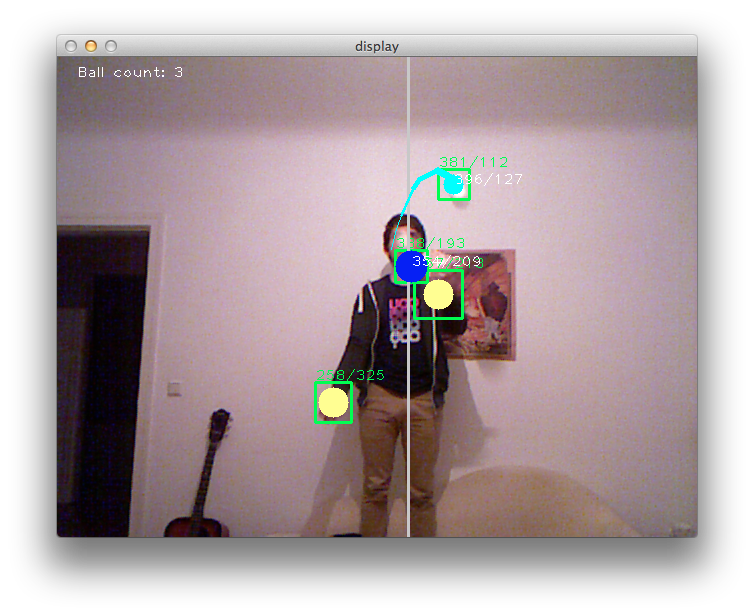
\includegraphics[scale=0.5]{img/ballcount-1.png}

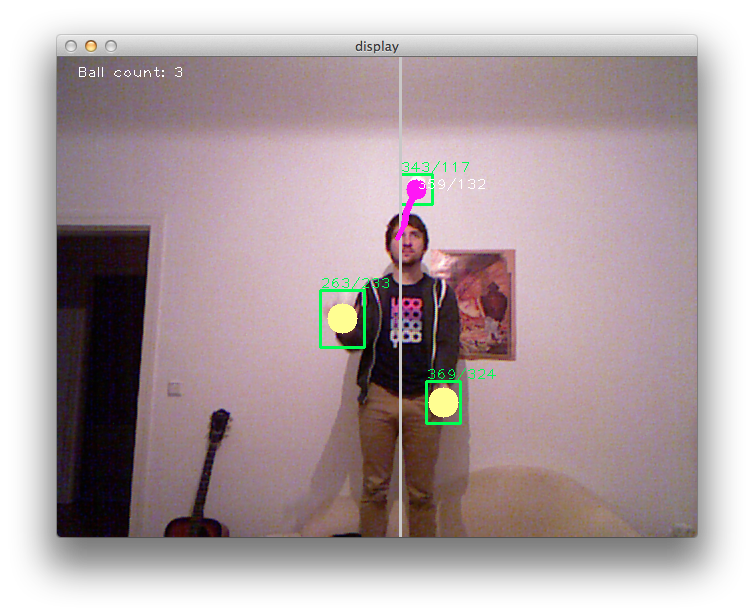
\includegraphics[scale=0.5]{img/ballcount-2.png}


\subsection{Würfe zählen}

\subsection{... ?}

\section{Fazit}

Lerneffekt, Frustration, Bewertung des Endprodukts


\newpage



\newpage
\phantomsection
\addcontentsline{toc}{section}{Quellen}
\renewcommand{\refname}{Quellen}
\bibliographystyle{plain}
\begin{thebibliography}{99}

%\cite{violajones}
\bibitem{hacking}
Jeff Kramer, Nicolas Burrus, Florian Echtler, Daniel Herrera C., Matt Parker\\
{\em Hacking the Kinect}\\
ISBN 978-1-4302-3867-6\\
Springer Science+Business Media New York, 2012.

% DIES IST EIN BEISPIELEINTRAG!
\bibitem{ole}
Ole Helvig Jensen,\\
{\em Implementing the Viola-Jones Face Detection Algorithm}\\
IMM-M.Sc.: ISBN 87-643-0008-0 \qquad ISSN 1601-233X\\
Technical University of Denmark, Informatics and Mathematical Modelling\\
Kongens Lyngby, Denmark, 2008.\\
\url{http://www.imm.dtu.dk/English/Research/Image_Analysis_and_Computer_Graphics/Publications.aspx?lg=showcommon&id=223656}

\bibitem{kober}
Jens Kober$^{1}$, Matthew Glisson, and Michael Mistry$^{2}$,\\
{\em Playing Catch and Juggling with a Humanoid Robot}.\\
Disney Research, Pittsburgh, USA,\\
$^{1}$ Bielefeld University, Germany,\\
$^{2}$ University of Birmingham, UK\\
FIXME.

\bibitem{openkinect}
{\em OpenKinect project}\\
\url{http://openkinect.org/wiki/Main_Page} (accessed on 2014-06-12).

\bibitem{libfreenect}
{\em libfreenect GitHub repository}\\
\url{https://github.com/OpenKinect/libfreenect} (accessed on 2014-06-12).

\end{thebibliography}

\end{document}
